
\documentclass[letterpaper,12pt]{article}
\usepackage[margin=1in]{geometry}
\geometry{letterpaper}
%\geometry{landscape} % Activate for for rotated page geometry
\usepackage[parfill]{parskip} % Activate to begin paragraphs with an
% empty line rather than an indent
\usepackage{amsfonts, amscd, amssymb, amsthm, amsmath}
\usepackage{mathtools} %xmapsto etc
\usepackage{pdfsync} %leaves makers for tex searching
\usepackage{enumerate}
\usepackage{graphicx,latexsym}
\graphicspath{{./pics}}
\usepackage{parskip}
\usepackage[
  backend=biber,
  style=alphabetic
]{biblatex}
\addbibresource{sources.bib}

%%% Color %%%---------------------------------------------------------
\usepackage{color}
\usepackage[dvipsnames]{xcolor}
\definecolor{dorange}{rgb}{.9,.3,0}
\definecolor{dgrey}{rgb}{.4,.4,.4}
\definecolor{plumb}{HTML}{8105C1}
\definecolor{pumpkin}{HTML}{E47604}
\definecolor{rose}{HTML}{C10091}
\definecolor{dgreen}{HTML}{25A75B}
\definecolor{dblue}{HTML}{0066FF}
\definecolor{cornflower}{HTML}{3256C3}
\definecolor{viridian}{HTML}{099A97}
\definecolor{alert}{HTML}{3256C3}

\newcommand\plumb[1]{{\color{plumb}#1}}
\newcommand\cornfl[1]{{\color{cornflower}#1}}
\newcommand\dgreen[1]{{\color{dgreen}#1}}
\newcommand\viridian[1]{{\color{viridian}#1}}
\newcommand\dblue[1]{{\color{dblue}#1}}
\newcommand\dred[1]{{\color{dred}#1}}
\newcommand\gray[1]{{\color{black!40}#1}}
\newcommand\black[1]{{\color{black}#1}}
\newcommand\pumpk[1]{{\color{pumpkin}#1}}
\newcommand\rose[1]{{\color{rose}#1}}

\newcommand{\NOTE}[1]{{\color{cornflower}#1}}
\newcommand{\alert}[1]{{\color{alert}#1}}
\newcommand{\Alert}[1]{\emph{\color{alert}#1}}

\renewcommand{\thefootnote}{\fnsymbol{footnote}}

%%% Theorems %%%---------------------------------------------------------
\theoremstyle{plain}
\newtheorem*{thm}{Theorem}
\newtheorem*{lemma}{Lemma}
\newtheorem*{prop}{Proposition}
\newtheorem*{cor}{Corollary}
\theoremstyle{definition}
\newtheorem*{defn}{Definition}
\newtheorem*{remark}{Remark}

%%% Environments %%%---------------------------------------------------------
\newenvironment{pf}{\color{black}\medskip
\paragraph*{\emph{Proof}.}}{\hfill \qedsymbol \medskip }
\newenvironment{ans}{\medskip \color{black}
\paragraph*{\emph{Answer}.}}{\hfill \break $~\!\!$ \dotfill \medskip }
\newenvironment{sketch}{\medskip \paragraph*{\emph{Proof sketch}.}}{ \medskip }
\newenvironment{summary}{\medskip \paragraph*{\emph{Summary}.}}{
\hfill \break \rule{1.5cm}{0.4pt} \medskip }
\newcommand\Ans[1]{$ $\hfill {\color{black}\emph{Answer:} {#1}}}
\newcommand{\Hint}[1]{{\small [\emph{Hint:} {#1}]}}

%%% Pictures %%%---------------------------------------------------------
%%% If you need to draw pictures, tikzpicture is one good option.
% Here are some basic things I always use:
\usepackage{tikz}
\usetikzlibrary{scopes}
\usepgflibrary{arrows}
\usepgflibrary{shapes}
\tikzstyle{V}=[draw, fill =black, circle, inner sep=0pt, minimum size=2pt]
\tikzstyle{bV}=[draw, fill =black, circle, inner sep=0pt, minimum size=4pt]
\tikzstyle{over}=[draw=white,double=black,line width=3pt]
\tikzstyle{C}=[draw, thick, fill =white, circle, inner sep=0pt,
minimum size=6pt]

\newcommand\TikZ[1]{
  \begin{matrix}
    \begin{tikzpicture}#1
    \end{tikzpicture}
\end{matrix}}

\newcounter{r}
\newcommand\Part[1]{
  \setcounter{r}{1}
  \foreach \x in {#1}{
    {\ifnum\value{r}=1
      \draw (0,\value{r}-1)--(\x,\value{r}-1);
    \fi}
    \draw (0,\value{r}) to (\x,\value{r});
    \foreach \y in {0, ..., \x} {\draw (\y,\value{r})--(\y,\value{r}-1);}
    \addtocounter{r}{1}
}}
\def\PartUNIT{.175}
%Self-contained tikz images for \Part above.
\newcommand{\PART}[1]{
  \begin{matrix}
    \begin{tikzpicture}[xscale=\PartUNIT, yscale=-\PartUNIT]
      \Part{#1}
    \end{tikzpicture}
  \end{matrix}
}

%%% Alphabets %%%---------------------------------------------------------
%%% Some shortcuts for my commonly used special alphabets and characters.
\def\cA{\mathcal{A}}\def\cB{\mathcal{B}}\def\cC{\mathcal{C}}\def\cD{\mathcal{D}}\def\cE{\mathcal{E}}\def\cF{\mathcal{F}}\def\cG{\mathcal{G}}\def\cH{\mathcal{H}}\def\cI{\mathcal{I}}\def\cJ{\mathcal{J}}\def\cK{\mathcal{K}}\def\cL{\mathcal{L}}\def\cM{\mathcal{M}}\def\cN{\mathcal{N}}\def\cO{\mathcal{O}}\def\cP{\mathcal{P}}\def\cQ{\mathcal{Q}}\def\cR{\mathcal{R}}\def\cS{\mathcal{S}}\def\cT{\mathcal{T}}\def\cU{\mathcal{U}}\def\cV{\mathcal{V}}\def\cW{\mathcal{W}}\def\cX{\mathcal{X}}\def\cY{\mathcal{Y}}\def\cZ{\mathcal{Z}}

\def\AA{\mathbb{A}} \def\BB{\mathbb{B}} \def\CC{\mathbb{C}}
\def\DD{\mathbb{D}} \def\EE{\mathbb{E}} \def\FF{\mathbb{F}}
\def\GG{\mathbb{G}} \def\HH{\mathbb{H}} \def\II{\mathbb{I}}
\def\JJ{\mathbb{J}} \def\KK{\mathbb{K}} \def\LL{\mathbb{L}}
\def\MM{\mathbb{M}} \def\NN{\mathbb{N}} \def\OO{\mathbb{O}}
\def\PP{\mathbb{P}} \def\QQ{\mathbb{Q}} \def\RR{\mathbb{R}}
\def\SS{\mathbb{S}} \def\TT{\mathbb{T}} \def\UU{\mathbb{U}}
\def\VV{\mathbb{V}} \def\WW{\mathbb{W}} \def\XX{\mathbb{X}}
\def\YY{\mathbb{Y}} \def\ZZ{\mathbb{Z}}

\def\fa{\mathfrak{a}} \def\fb{\mathfrak{b}} \def\fc{\mathfrak{c}}
\def\fd{\mathfrak{d}} \def\fe{\mathfrak{e}} \def\ff{\mathfrak{f}}
\def\fg{\mathfrak{g}} \def\fh{\mathfrak{h}} \def\fj{\mathfrak{j}}
\def\fk{\mathfrak{k}} \def\fl{\mathfrak{l}} \def\fm{\mathfrak{m}}
\def\fn{\mathfrak{n}} \def\fo{\mathfrak{o}} \def\fp{\mathfrak{p}}
\def\fq{\mathfrak{q}} \def\fr{\mathfrak{r}} \def\fs{\mathfrak{s}}
\def\ft{\mathfrak{t}} \def\fu{\mathfrak{u}} \def\fv{\mathfrak{v}}
\def\fw{\mathfrak{w}} \def\fx{\mathfrak{x}} \def\fy{\mathfrak{y}}
\def\fz{\mathfrak{z}}
\def\fN{\mathfrak{N}}
\def\fgl{\mathfrak{gl}}  \def\fsl{\mathfrak{sl}}
\def\fso{\mathfrak{so}}  \def\fsp{\mathfrak{sp}}
\def\GL{\mathrm{GL}} \def\SL{\mathrm{SL}}
\def\SP{\mathrm{SL}}\def\OG{\mathrm{O}}

\def\aa{\mathbf{a}} \def\bb{\mathbf{b}} \def\cc{\mathbf{c}}
\def\dd{\mathbf{d}} \def\ee{\mathbf{e}} \def\ff{\mathbf{f}}
%\def\gg{\mathbf{g}}
\def\hh{\mathbf{h}} \def\ii{\mathbf{i}} \def\jj{\mathbf{j}} \def\kk{\mathbf{k}}
%\def\ll{\mathbf{l}}
\def\mm{\mathbf{m}} \def\nn{\mathbf{n}} \def\oo{\mathbf{o}}
\def\pp{\mathbf{p}} \def\qq{\mathbf{q}} \def\rr{\mathbf{r}}
\def\ss{\mathbf{s}} \def\tt{\mathbf{t}} \def\uu{\mathbf{u}}
\def\vv{\mathbf{v}} \def\ww{\mathbf{w}} \def\xx{\mathbf{x}}
\def\yy{\mathbf{y}} \def\zz{\mathbf{z}}
\def\zzero{\mathbf{0}}

\def\<{\langle} \def\>{\rangle}
\def\Aut{\mathrm{Aut}}
\def\ch{ \stackrel}
\def\col{\mathrm{col}}
\def\dim{\mathrm{dim}}
\def\End{\mathrm{End}}
\def\ev{\mathrm{ev}}
\def\f{\varphi}
\def\gcd{\mathrm{gcd}}
\def\half{\hbox{$\frac12$}}
\def\Hom{\mathrm{Hom}}
\def\img{\mathrm{img}}
\def\id{\mathrm{id}}
\def\Inn{\mathrm{Inn}}
\def\lcm{\mathrm{lcm}}
\def\normeq{\trianglelefteq}
%\def\ch{ \stackrel{\mathrm{ch}}{\trianglelefteq}}
%\def\normeq{\trianglelefteq}
\def\nul{\mathrm{nullity}}
\def\row{\mathrm{row}}
\def\rk{\mathrm{rank}}
\def\sgn{\mathrm{sgn}}
\def\sp{\mathrm{span}}
\def\supp{\mathrm{supp}}
\def\Syl{\mathrm{Syl}}
\def\tr{\mathrm{tr}}
\def\vep{\varepsilon}

\usepackage{mathabx}
\def\acts{\lefttorightarrow} %group action

%\usepackage{mathtools}
\usepackage{wasysym}
\makeatletter
\let\NAT@parse\undefined
\makeatother
\usepackage{hyperref} %[pdftex,bookmarks]
\hypersetup{
  colorlinks=true,
  linkcolor=viridian,
  filecolor=viridian,
  citecolor=viridian,
  urlcolor=viridian,
  pdfpagemode=FullScreen,
}

\def\ol{\overline}
\newcommand{\Mod}[1]{\ (\mathrm{mod}\ #1)}

\def\Hfill{$ $\hfill}

% Arrows:
\newcommand\xdhrightarrow[2][]{%
  \mathrel{\ooalign{$\xrightarrow[#1\mkern4mu]{#2\mkern4mu}$\cr%
  \hidewidth$\rightarrow\mkern4mu$}}
}
%\newcommand\dhrightarrow{%
% \mathrel{\ooalign{$\rightarrow$\cr%
% $\mkern3.5mu\rightarrow$}}
%}
\def\dhrightarrow{\twoheadrightarrow}
\def\dhleftarrow{\twoheadleftarrow}

% Arrays:
\newcommand\Pmatrix[1]{
  \begin{pmatrix}#1
\end{pmatrix}}
\newcommand\smatrix[1]{\text{\small$
    \begin{pmatrix}#1
\end{pmatrix}$}}
\newcommand\fmatrix[1]{\text{\footnotesize$
    \begin{pmatrix}#1
\end{pmatrix}$}}
\newcommand\tmatrix[1]{\text{\tiny$
    \begin{pmatrix}#1
\end{pmatrix}$}}
\newcommand{\linespace}{[5pt]}
\newcommand\tx[1]{\texttt{#1}}

\makeatletter
\newcommand{\chareq}{%
  \mathrel{\mathpalette\chRAW\relax}%
}

\newcommand{\chRAW}[2]{%
  \sbox\z@{$#1\LHD$}%
  \sbox\tw@{$#1\leqslant$}%
  \dimen@=\ht\tw@
  \advance\dimen@-\ht\z@
  \advance\dimen@ .3pt
  \ifx#1\displaystyle
  \advance\dimen@ .2pt
  \else
  \ifx#1\textstyle
  \advance\dimen@ .2pt
  \fi
  \fi
  \ooalign{\raisebox{\dimen@}{$\m@th#1\LHD$}\cr$\m@th#1\leqslant$\cr}%
}
\makeatother
\allowdisplaybreaks
\setlength{\parindent}{20pt}
\setlength{\parskip}{3pt}
\fontsize{12}{13.5}

%%%%%%%%%%%%%%%%%%%%%%%%%%%%%%
%%%%%%%%%%%%%%%%%%%%%%%%%%%%%%

\title{CSCI 378 Final Project Writeup}
\author{Bram Schuijff}

\begin{document}
\clearpage\maketitle
\thispagestyle{empty}

\section{Background Research}

Prior to implementing any networks, I originally tried to examine
physics-informed neural networks (PINNs). I read both research papers which
introduced the idea and parsed the PINN library itself. Unfortunately, I
abandoned this idea due to the amount of physics and partial differential
equation knowledge it required, both of which I am lacking in. I also lacked an
interesting dataset on which I could actually train a PINN, and I did not know
where to start looking for such a dataset.

The majority of my background research following my abandonment of PINNs was in
trying to figure out how to implement recurrent neural networks.  Most of this
implementation occurred before we went over temporal convolutional networks in
class. Therefore, I had to sift through Torch documentation to figure out how
they worked. This started with trying LSTM networks and, when I realized they
were overkill for the job and took far too long to train, moving to temporal
convolutional networks.

Another piece of research I had to do was figuring out precisely which dataset
to use. There were a few options such as NASA's Daymet dataset, but I
eventually decided on UC Berekeley's temperature anomaly dataset. This is
because I had a very hard time trying to adapt the Daymet dataset to a machine
learning context due to the complex geospatial file type. Additionally, due to
the dataset's size, training networks took a ridiculously long time even on
Weftdrive.

\section{The Problem}

The main problem I am attempting to solve is to predict daily temperature
anomalies. Based on the historic mean temperature of the planet, how much did
the global temperature of that day deviate from that mean? UC Berkeley has a
dataset with temperature anomaly information for each day between 1880 and
September 2022. My goal was to use this dataset to train a network which could
predict future temperature anomalies. In this sense, I was looking at a time
series forecasting problem. This problem is of practical interest because it
can demonstrate the impact of climate change on the average temperature of our
planet over time. Additionally, this network could predict the future impacts
of climate change.

\section{Implementation}

I implemented a temporal convolutional network. I did this as opposed to an
LSTM network for a few reasons: the number of parameters in a
moderately-complex LSTM caused horrific overfitting on my low-dimensional
dataset, LSTM networks had ludicrous file sizes that made debugging them
painful, and they took far too long to train. Furthermore, I saw very little
difference in performance between an LSTM network and the much smaller temporal
convolutional network, making the latter the obvious choice.

The network itself is relatively simple, accepting an argument \tx{layers} in
its constructor which is a list of positive integers. The network then contains
a number of hidden temporal convolutional layers equal to the length of the
list and where each layer has a number of output channels in accordance with
its associated list element. Each layer also has a \tx{ReLU} activation
function and one-dimensional padding in accordance with what we went over in
class. The layers also get increasingly dilated as we go down the hidden
layers, allowing for the network to observe more of its context window at once.
Finally, our classifier is just a kernel of size $1$ which converts our data
into a prediction for our time series with $1$ channel corresponding to the
real number we are trying to predict.

I have two implementations for what our predictions are supposed to model.
Given a context window of size $k$, we either attempt to predict the element
immediately following our context window or we attempt to predict the $k$
elements following our context window. One of these problems is clearly harder
than the other as the first is a sub-problem of the second. The way that I
implemented this is with a global boolean variable called \tx{predictive}. If
it is \tx{False}, we only attempt to predict the next element. If it is
\tx{True}, we attempt to predict the entire next context window.
\tx{predictive} is read in the \tx{TempAnomalyDataset} object which is a
subclass of the \tx{torch.Dataset} object which is how we actually load our
data.

I started with the next-element case but quickly found that it overfit with
even tiny models. Additionally, it was very bad at producing predictions for
future temporal anomaly data on even small cases because it often got into
feedback loops as it was fed its own predictions to forecast the time series. I
then moved to the full context window case which, while it took longer to
train, produced significantly more desirable models for my use case.
Overfitting became much less of an issue because of the increasing difficulty
of the problem. Additionally, this framework did not require the network to be
fed its own inputs in order to forecast the time series; instead, we gave it a
tail of the input data which it used to produce an equally-sized forecast.

The final piece of our implementation is some simple \tx{matplotlib} code which
allows us to visualize our predictions. This can be found in the \tx{vis.py}
file where blue represents our real dataset, red represents our predictions
over the dataset, and yellow represents our forecast.

\section{Results}

My models were able to pretty accurately predict the dataset with minimal
overfitting even at very large network sizes. I tested this with Tensorboard
and varied my architecture, learning rate and weight decay to achieve optimal
results. For smaller architectures, it seems that high epoch ranged work best
with a relatively high learning rate. These architectures are able to
continually learn for long periods of time with their validation losses
steadily decreasing. In the end, a MSE loss of approximately $0.08$ was about
as good as I could get. Figure~\ref{accurate} demonstrates that our network was
able to accurately predict data within the dataset.

\begin{figure}[ht]
  \begin{center}
    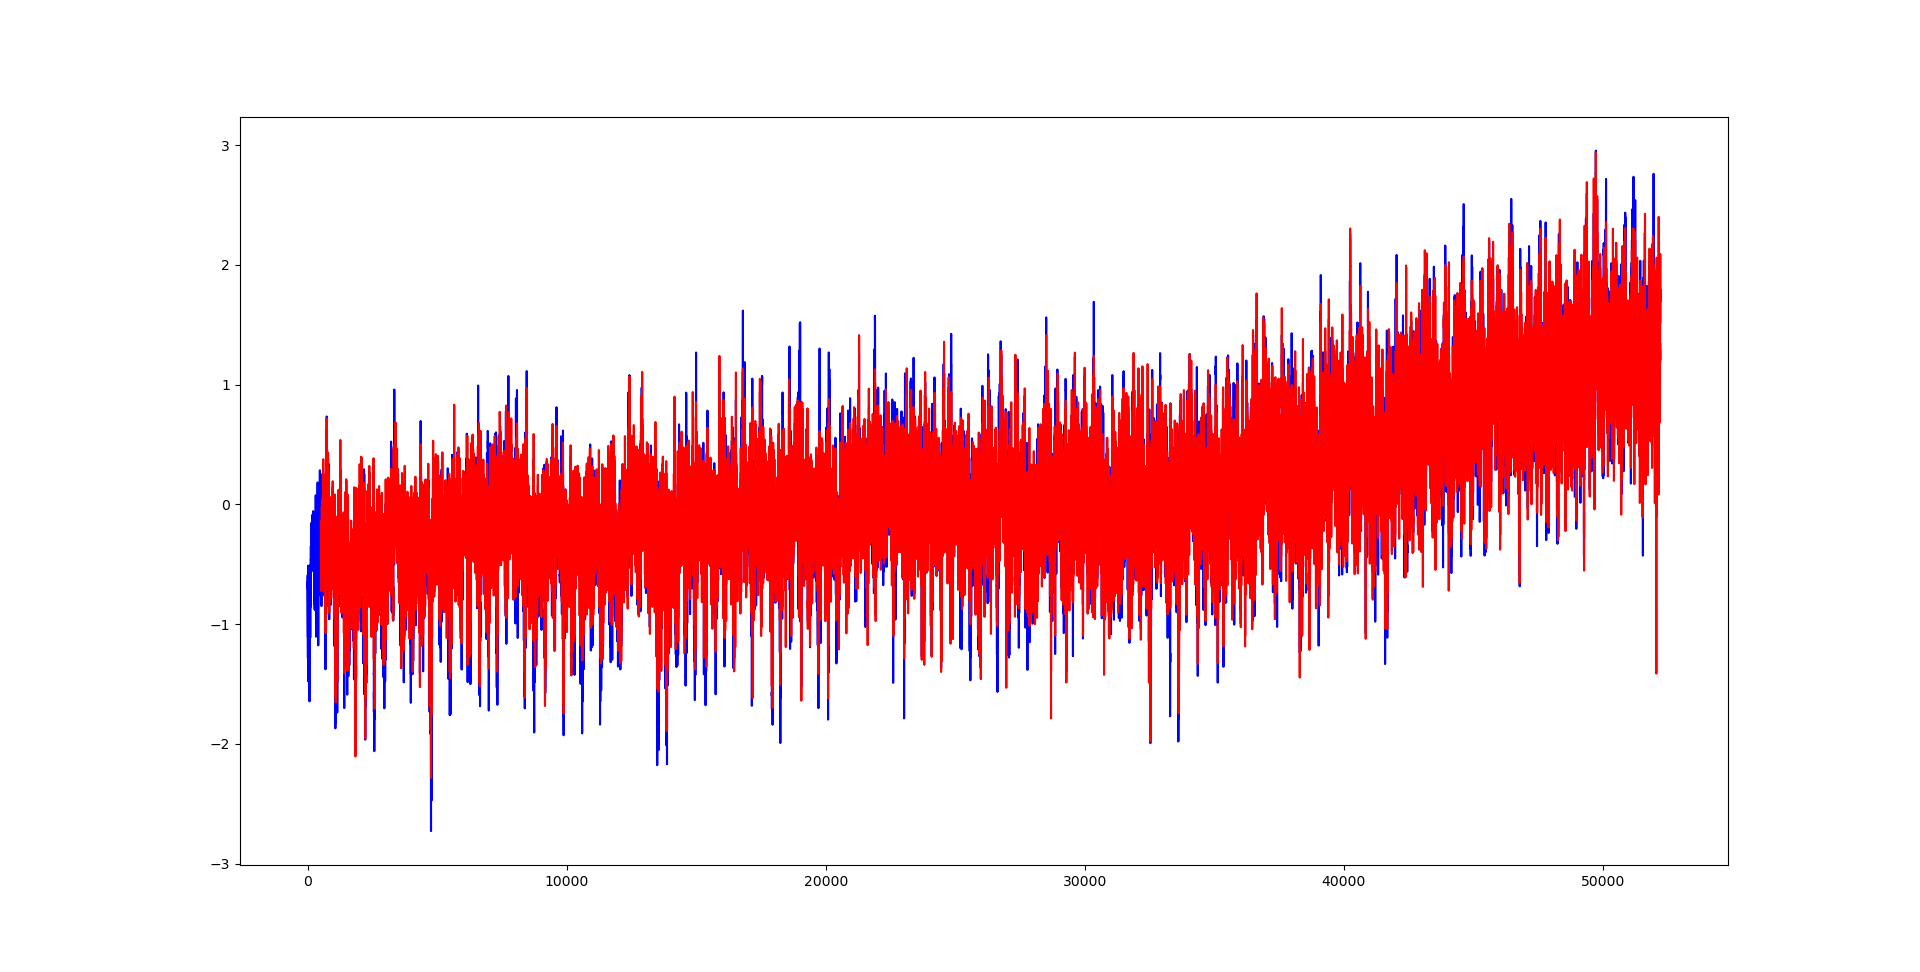
\includegraphics[scale=0.27]{accurate_predictions.png}
    \caption{Relatively large architecture demonstrating accurate predictions}
    \label{accurate}
  \end{center}
\end{figure}

Unfortunately, despite this relatively good loss, my forecasting left a lot to
be desired. It seems that no matter how small of a window I asked my networks
to forecast, they were simply incapable of producing good results. I tried
everything I could think of to get good results and nevertheless, my results
were lacking. Larger networks had a tendency to squash they predictions in a
very small range of values while smaller networks would have extremely erratic
predictions. Evidence for both cases is provided in Figures~\ref{squash}
and~\ref{erratic}.

\begin{figure}[ht]
  \begin{center}
    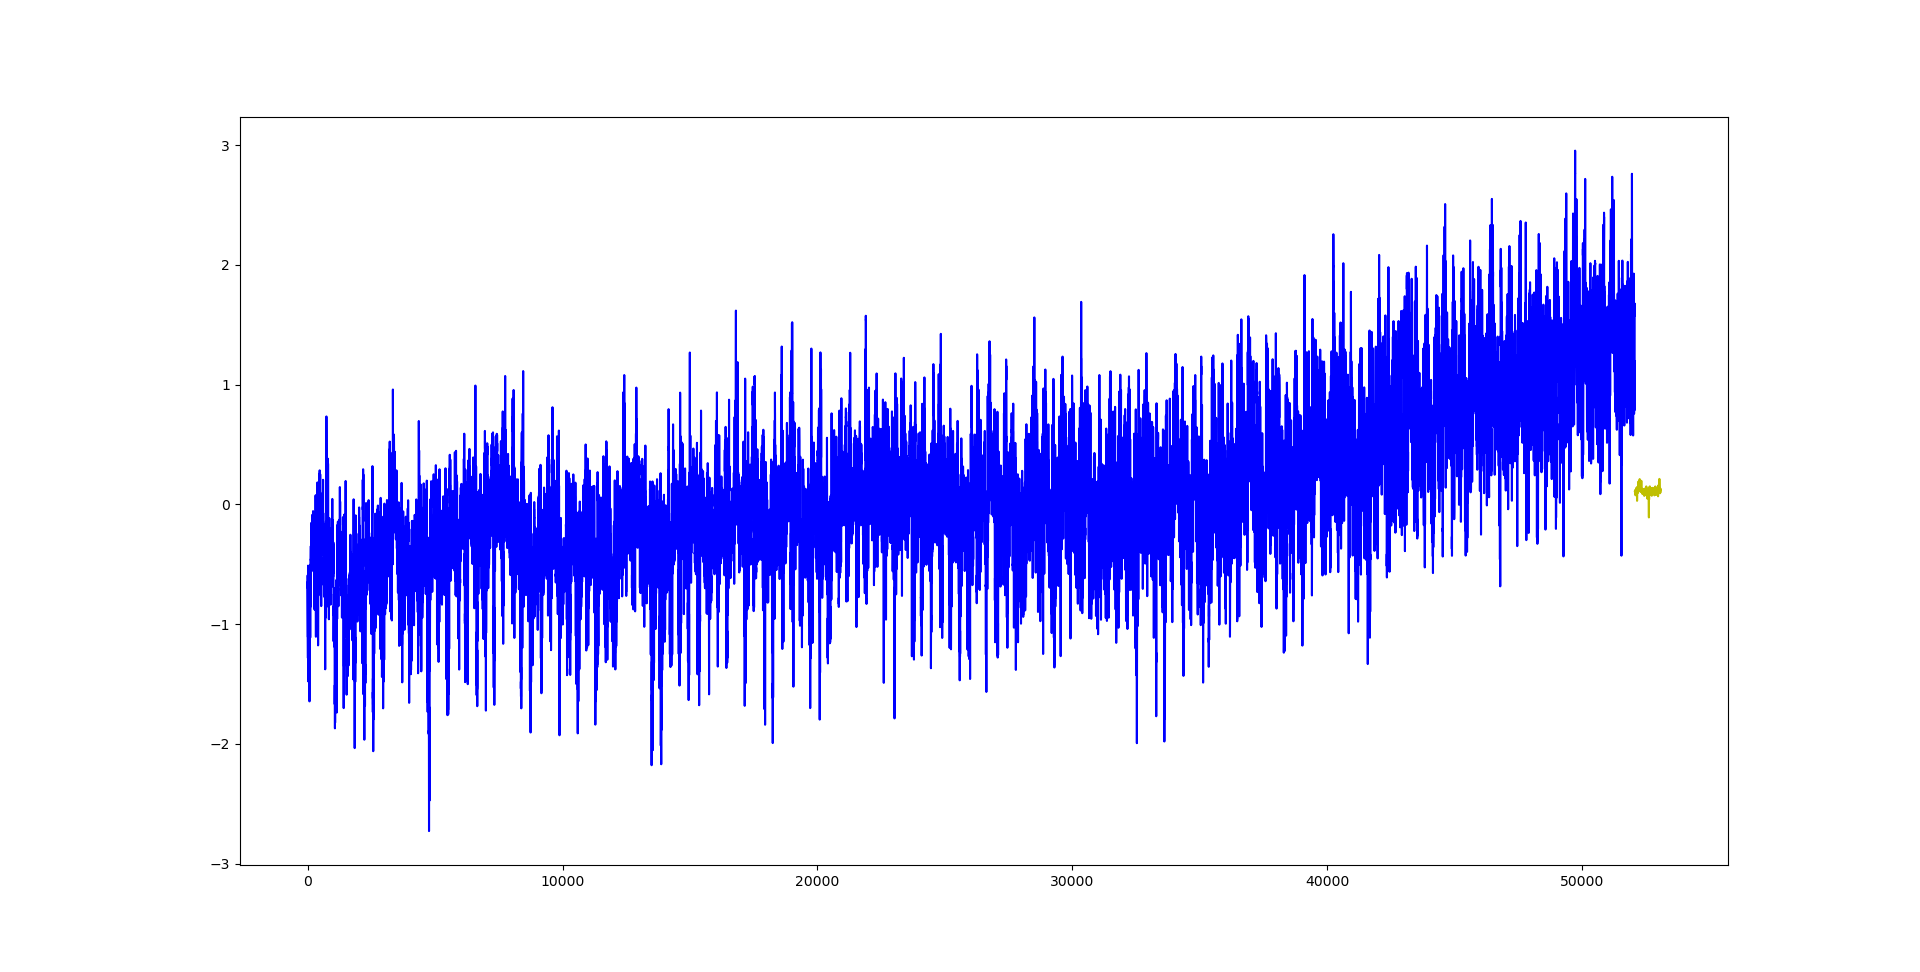
\includegraphics[scale=0.27]{squash_predictions.png}
    \caption{Large architecture demonstrating squashed predictions}
    \label{squash}
  \end{center}
\end{figure}

\begin{figure}[ht]
  \begin{center}
    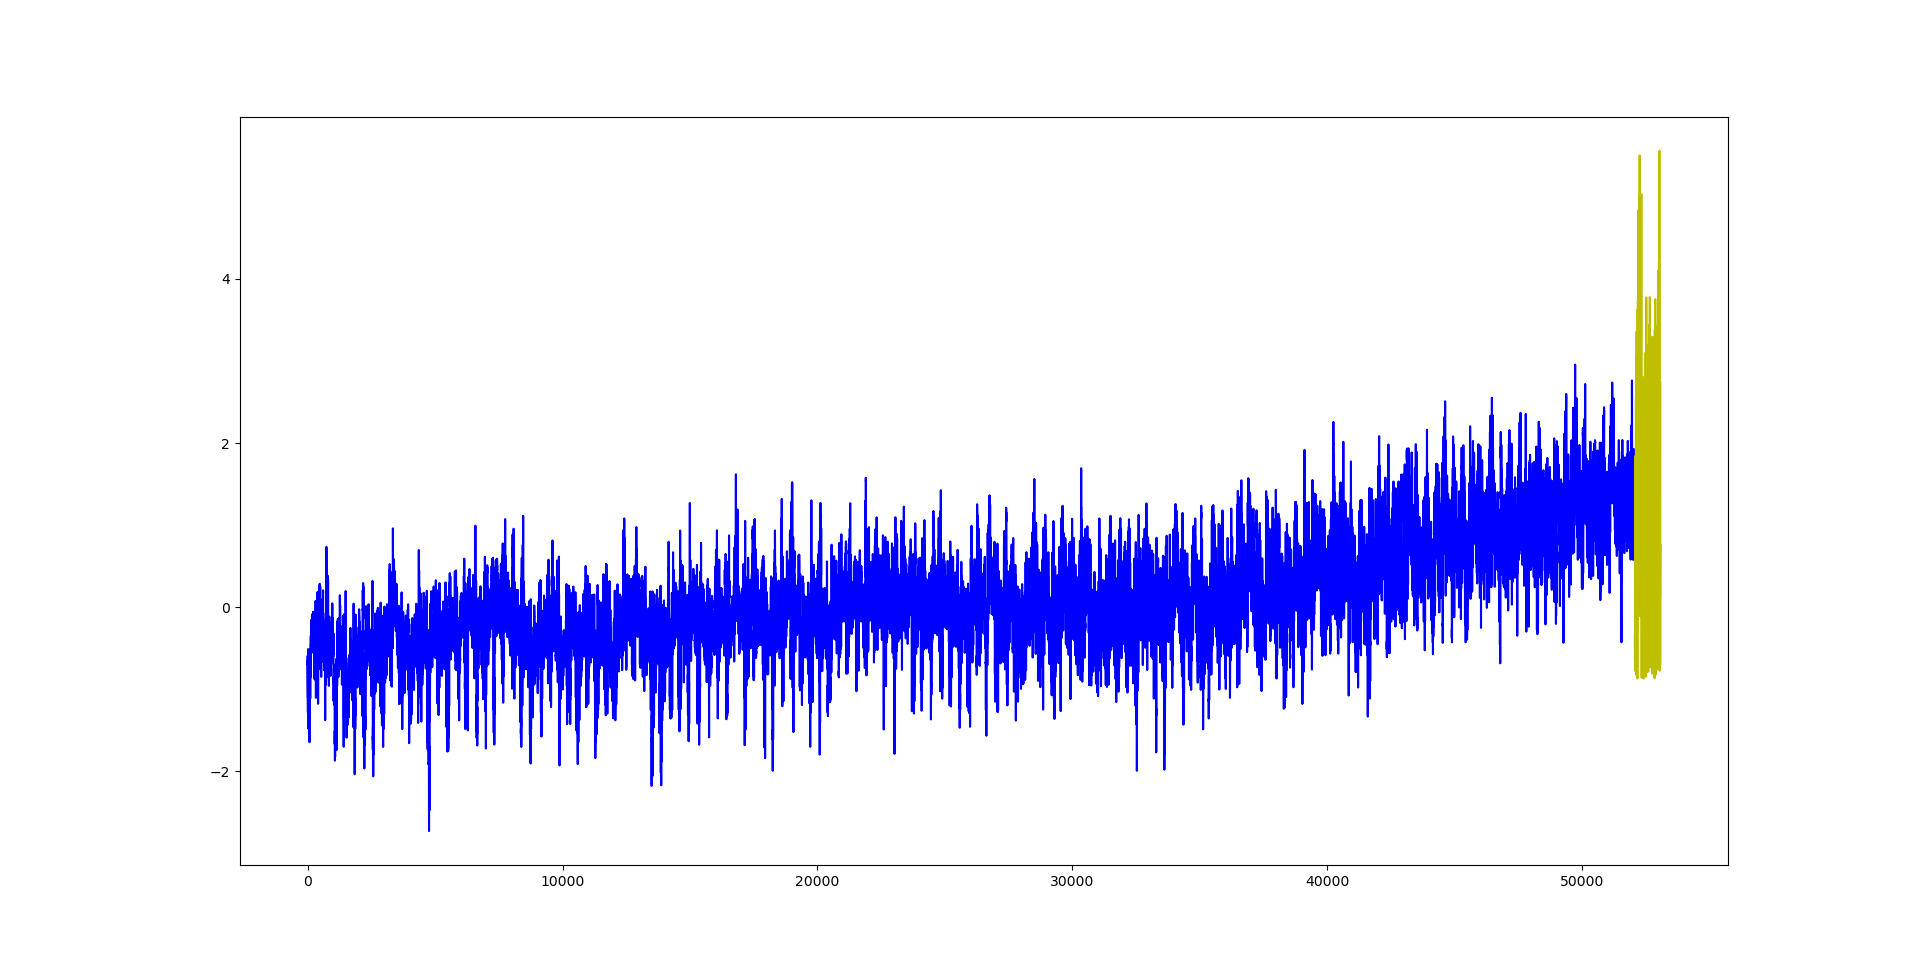
\includegraphics[scale=0.27]{erratic_predictions.png}
    \caption{Small architecture demonstrating erratic predictions}
  \end{center}
  \label{erratic}
\end{figure}

In the above figures, the blue line represents our real dataset and the yellow
line represents the model's forecast. These are both demands for the model to
forecast the next $1000$ days of temperature anomalies. The smaller model has
predicitons which are all over the place while the larger model tends to squash
its values just above $0$. I cannot for the life of me figure out why this is
the case and I have not been able to fix it. There appears to be no
middle-ground between wildly erratic predictions and completely squashed
predictions. Even when a model demonstrates good behavior over the validation
set, this behavior persists. Perhaps it is because of how I am getting the
model to forecast, but I have not been able to root out the source of the bug.

\end{document}
